%!TEX root = Manuscrit.tex

\chapter{Introduction}
\label{chap:intro}
\minitoc

\section{Exemple d'illustration}

\subsection{Une sous section pour le fun}

Eh non je n'écrirai pas votre manuscrit... Juste pour montrer que ce style gère les accents et comment on inclut une figure. A noter, les path vers les dossiers d'images de départ sont définis dans formatAndDefs.tex . Pensez à bien ouvrir et sauvegarder vos fichiers en UTF-8 pour conserver les accents.

\begin{figure}[!htbp]
  \begin{center}
    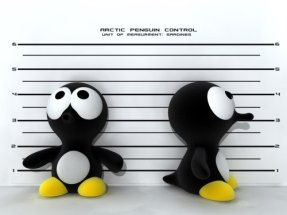
\includegraphics[width=0.9\textwidth]{Chapitre1/arctic_control}
  \end{center}
  \caption{Une jolie image...}
  \label{fig:jolieImage}
\end{figure}

\section{Une équation}

Juste pour montrer les commandes argmin et dérivée partielle.

\begin{equation}
  T = \argmin_T E(T,R,F)
\end{equation}

Régularisation :

\begin{equation}
  \pd{T}{t} = \Delta T
\end{equation}

\section{Une autre section}

Pour montrer l'environnement bulletList

\begin{bulletList}
 \item Premier point
 \item Deuxième point
 \item Et un acronyme utilisé (défini dans Acronymes.tex) \ac{DTI}
\end{bulletList}
